\documentclass[12pt,a4paper]{article}

% Packages
\usepackage[utf8]{inputenc}
\usepackage[T1]{fontenc}
\usepackage[english]{babel}
\usepackage{amsmath, amssymb}
\usepackage{tikz}
\usepackage{enumitem}
\usepackage{float}
\usepackage{caption}
\usepackage{graphicx}
\usepackage[margin=2.5cm]{geometry}

\title{Problem R28: Viscous Flow in Combined Pipe and Hull System}
\author{}
\date{}

\begin{document}

\maketitle

\begin{figure}[H]
\centering
    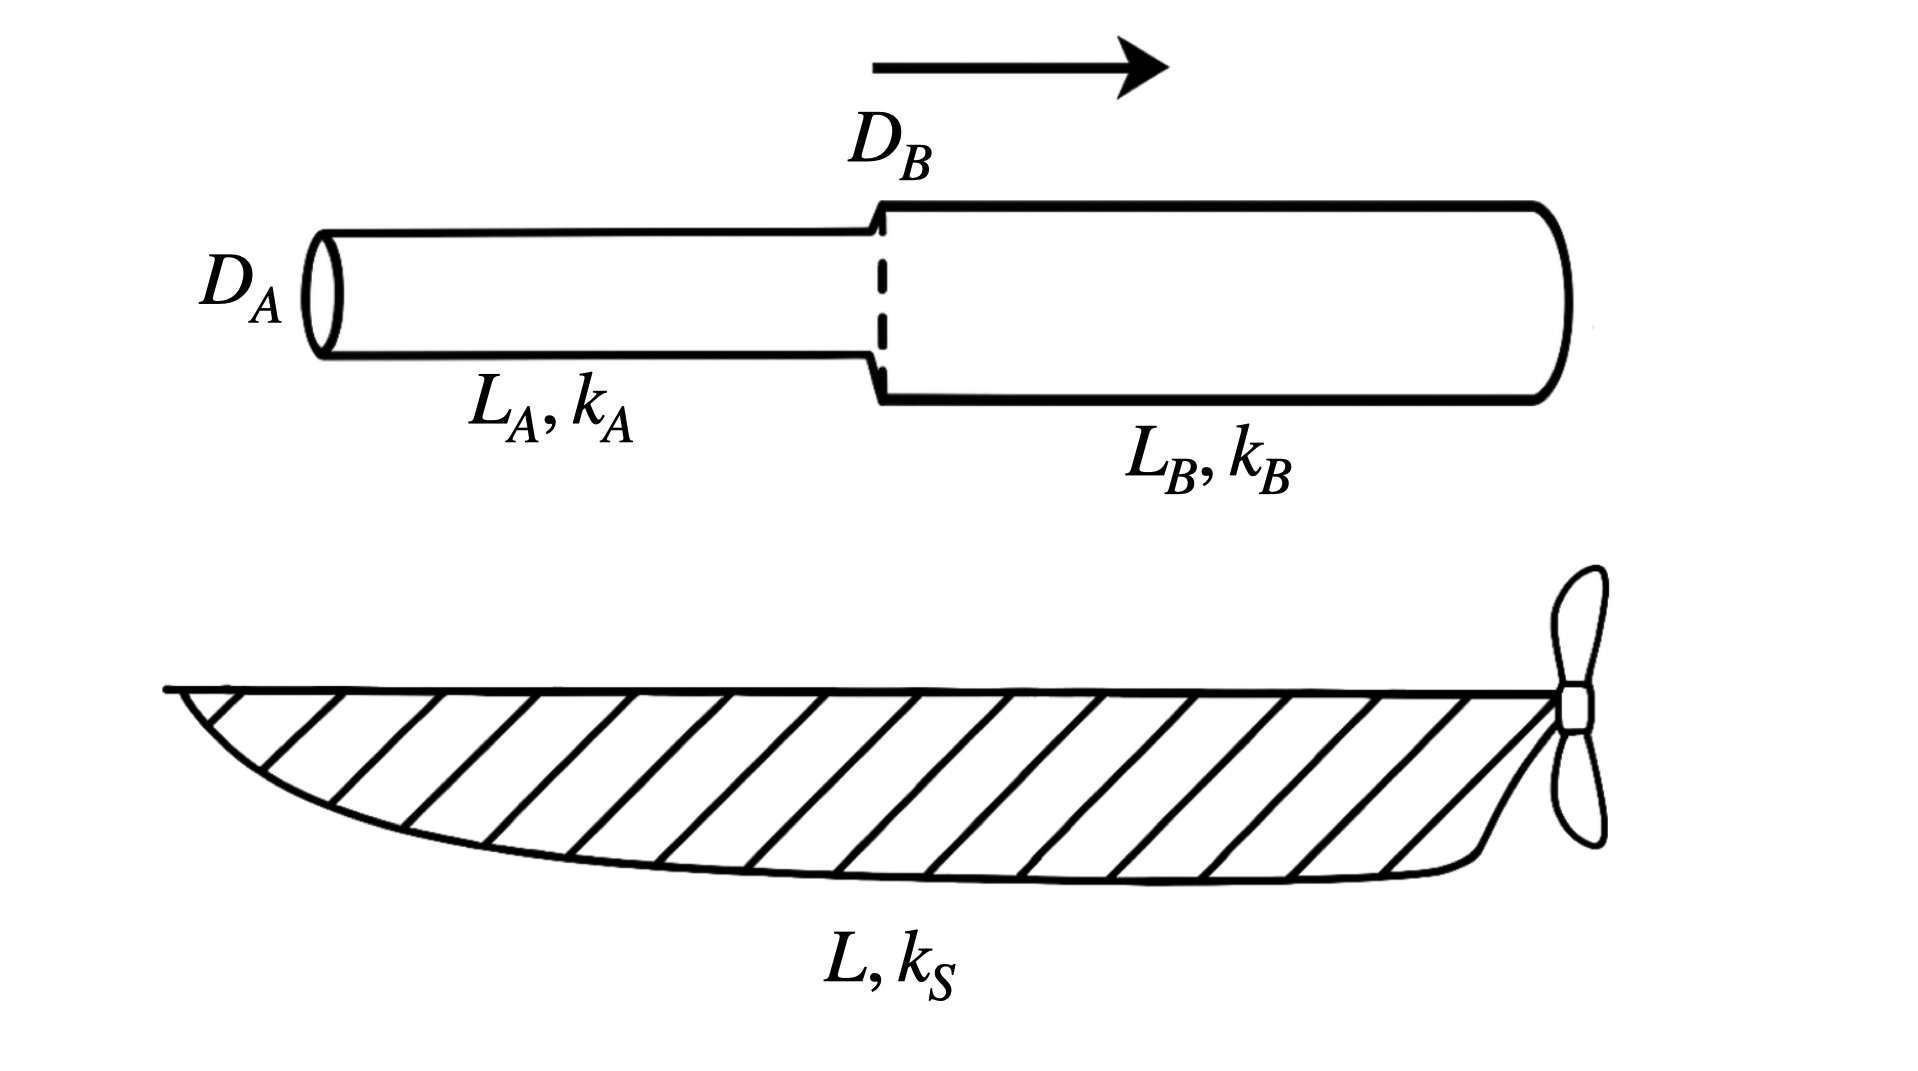
\includegraphics[width=0.9\textwidth]{HullSketch.png}
\caption{Sketch of the research vessel's hull and propulsion system. The vessel has a hybrid propulsion system with a conventional propeller and a water discharge system through two serial pipe sections.}
\end{figure}

\section*{Scenario}
A research vessel uses a hybrid propulsion system composed of:
\begin{itemize}
    \item a conventional propeller system, and
    \item a water discharge system that ejects seawater through two \textbf{serial} pipe sections (see sketch).
\end{itemize}
The system is designed such that all pipe flow is \textbf{tripped to turbulent regime at the inlet}. The outer hull flow is also assumed \textbf{fully turbulent}, avoiding laminar-transition complexity.

Assume seawater at density $\rho = 1025\,\mathrm{kg/m^3}$ and kinematic viscosity $\nu = 1.1 \times 10^{-6}\,\mathrm{m^2/s}$.

\paragraph{Pipe Sections:}
\begin{itemize}
    \item Section A: length $L_A = 30\,\mathrm{m}$, diameter $D_A = 0.3\,\mathrm{m}$, roughness $k_A = 0.3\,\mathrm{mm}$
    \item Section B: length $L_B = 20\,\mathrm{m}$, diameter $D_B = 0.2\,\mathrm{m}$, roughness $k_B = 1.2\,\mathrm{mm}$
\end{itemize}
Total volumetric flow rate: $Q = 0.08\,\mathrm{m^3/s}$

\paragraph{Hull Geometry:}
\begin{itemize}
    \item Length $L = 85\,\mathrm{m}$
    \item Draft $T = 6\,\mathrm{m}$
    \item Roughness $k_s = 4\,\mathrm{mm}$
\end{itemize}
Assume the \textbf{wetted area} is approximately $A = 2 \cdot L \cdot T$ (i.e. both vertical sides only).

Ship velocity: $V = 9\,\mathrm{m/s}$ \\
Propeller efficiency: $\eta_S = 0.78$

\section*{Solutions}
\begin{enumerate}[label=\alph*)]
    \item Mean velocity:
    \[
    u_A = \frac{Q}{A_A} = \frac{0.08}{\pi (0.15)^2} \approx 1.13 \, \mathrm{m/s}, \quad
    u_B = \frac{Q}{A_B} = \frac{0.08}{\pi (0.1)^2} \approx 2.55 \, \mathrm{m/s}
    \]

    \item Reynolds number:
    \[
    Re_A = \frac{u_A D_A}{\nu} \approx \frac{1.13 \cdot 0.3}{1.1 \times 10^{-6}} \approx 3.1 \times 10^5 \, (\text{turbulent}),
    \quad Re_B \approx 4.6 \times 10^5 \, (\text{turbulent})
    \]

    \item Friction factors (fully rough):
    \[
    \lambda_A = \left(\frac{1}{1.74 - 2 \log_{10}(2 \cdot 0.0003 / 0.3)}\right)^2 \approx 0.025,
    \quad \lambda_B \approx 0.035
    \]
    \[
    \Delta p_V = \sum \left( \lambda_i \frac{L_i}{D_i} \frac{\rho}{2} u_i^2 \right) \approx 0.025 \cdot \frac{30}{0.3} \cdot \frac{1025}{2} (1.13)^2 + 0.035 \cdot \frac{20}{0.2} \cdot \frac{1025}{2} (2.55)^2 \approx 34.6 + 296.8 = 331.4 \, \mathrm{Pa}
    \]

    \item Hull friction:
    \[
    c_f = \left(1.89 + 1.62 \cdot \log_{10}\left(\frac{85}{0.004}\right)\right)^{-2.5} \approx 0.0034
    \]
    Wetted area: $A = 2LT = 2 \cdot 85 \cdot 6 = 1020 \, \mathrm{m^2}$
    \[
    F = c_f \cdot \frac{1}{2} \rho V^2 A \approx 0.0034 \cdot 0.5 \cdot 1025 \cdot 81 \cdot 1020 \approx 143{,}950 \, \mathrm{N}
    \]

    \item Total power:
    \[
    P = \frac{F \cdot V + Q \cdot \Delta p_V}{\eta_S} = \frac{143950 \cdot 9 + 0.08 \cdot 331.4}{0.78} \approx \frac{1.295 \times 10^6 + 26.5}{0.78} \approx 1.66 \times 10^6 \, \mathrm{W} = 1660 \, \mathrm{kW}
    \]
\end{enumerate}

\end{document}
